\chapter[TRANSFORMAÇÃO DE COORDENADAS]{TRANSFORMAÇÃO DE COORDENADAS}

Na transformação de coordenadas, é necessário conhecer em quais parâmetros estão embutidas as informações da forma e do tamanho real do domínio de cálculo. Existem duas abordagens na transformação de coordenadas:
\begin{itemize}
    \item o sistema de coordenada local (relacionado a malhas não-estruturadas)
    \item sistema de coordenadas global (relacionado a malhas estruturadas)
\end{itemize}

Seja $f=f(\xi, \eta)$, onde $f$ reqpresenta $x,y,T$\dots
Neste caso:

\begin{equation}
    \frac{\partial f}{\partial x} = \frac{\partial f}{\partial \xi}\frac{\partial \xi}{\partial x}+\frac{\partial f}{\partial \eta}\frac{\partial \eta}{\partial x}
    \label{eq:2.1}
\end{equation}
\begin{equation}
    \frac{\partial f}{\partial y} = \frac{\partial f}{\partial \xi}\frac{\partial \xi}{\partial y}+\frac{\partial f}{\partial \eta}\frac{\partial \eta}{\partial y}
    \label{eq:2.2}
\end{equation}

Fazendo $f=x$ na equação \ref{eq:2.1} e $f=y$ na equação \ref{eq:2.2}, obtém-se:
\begin{equation*}
    1 = x_\xi \xi_x + x_\eta \eta_x\\
    0 = y_\xi \xi_x + y_\eta \eta_x
\end{equation*}

Resolvendo o sistema anterior encontra-se:
\begin{equation}
    \label{eq:2.3}
    \xi_x = y_\eta J
\end{equation}
\begin{equation}
    \label{eq:2.4}
    \eta_x = -y_\xi J
\end{equation}

\begin{equation}
    J = (x_\xi y_\eta - x_\eta y_\xi)^(-1)
    \label{eq:2.5}
\end{equation}

Onde na equação \ref{eq:2.5} $J$  é o jacobiano da transformação do sistema de coordenadas.

Agora, fazendo-se $f=x$ em \ref{eq:2.2} e $f=y$ em \ref{eq:2.2}, tem-se:
\begin{equation*}
    0 = x_xi \xi_y + x_\eta \eta_y
    1 = y_\xi \xi_y + y_\eta \eta_y
\end{equation*}

Ao se resolver o sistema anterior, obtém-se:
\begin{equation}
    \label{eq:2.6}
    \xi_y = -x_\eta J
\end{equation}
\begin{equation}
    \label{eq:2.7}
    \eta_y = x_\xi J
\end{equation}

A matriz jacobiana da transformação de coordenadas é definida por:
\begin{equation}
    \label{eq:2.8}
    J =
    \begin{bmatrix}
        \xi_x & \xi_y\\
        \eta_x & \eta_y
    \end{bmatrix}
    = (\xi_x \eta_y - \xi_y \eta_x)
\end{equation}

Tanto o Jacobiano quanto as métricas de transformação $(\xi_x, \xi_y, \eta_x, \eta_y)$ aparecerão nas equações diferenciais quando estas forem transformadas para o novo sistema de coordenadas $(\xi,\eta)$.

Como os domínios são discretos, existem dificuldades em se calcular as métricas da transformação direta $(\xi_x, \xi_y, \eta_x, \eta_y)$. Exemplo:

$\xi_x=\frac{\partial \xi}{\partial x}$ é necessário conhecer a variação $\partial x$ em uma linha de $y$ constante.

Desde modo, para se contornar esta dificuldade, utilizam-se as métricas da transformação inversa $(x_\xi, x_\eta, y_\xi, y_\eta)$, uma vez que no espaço transformado $(\xi, \eta)$ todas as coordenadas são conhecidas a priori.

As relações entre as métricas da transformação direta e inversa são dadas pelas equações \ref{eq:2.3} e \ref{eq:2.4}, \ref{eq:2.6} e \ref{eq:2.7}.

O jacobiano da transformação inversa é dado por:

\begin{equation}
    \label{eq:2.9}
    J^{-1} =
    \begin{vmatrix}
        x_\xi & x_\eta\\
        y_\xi & y_\eta
    \end{vmatrix}
    = (x|xi y_\eta - x|eta y_xi)
\end{equation}

Substituindo-se as equações \ref{eq:2.3}, \ref{eq:2.4}, \ref{eq:2.6} e \ref{eq:2.7} na equação \ref{eq:2.9}, prova-se que:

\begin{equation}
    \label{eq:2.10}
    J = \frac{1}{J^{-1}}
\end{equation}

Conforme a figura \ref{fig:transformacao} podemos chegar nas seguintes relações:
\begin{figure}[]
    \centering
    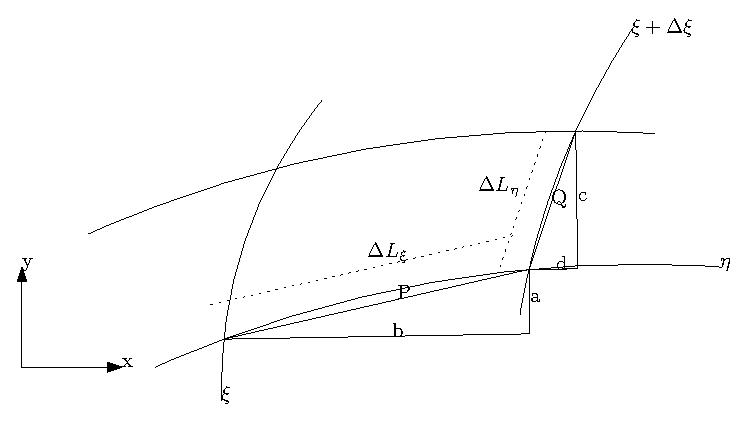
\includegraphics{fig/transformacao.eps}
    \label{fig:transformacao}
    \caption{Transformação de Coordenadas}
\end{figure}

\begin{equation*}
    x_\xi \vert_P = \frac{x(\xi+\Delta \xi)-x(\xi)}{\Delta \xi} = \frac{b}{\Delta \xi}
\end{equation*}

Ou seja, $b=x_\xi \Delta \xi$

\begin{equation*}
    y_\xi \vert_P = \frac{y(\xi+\Delta \xi)-y(\xi)}{\Delta \xi} = \frac{a}{\Delta \xi}    
\end{equation*}

Ou seja, $a=y_\xi \Delta \xi$

\begin{equation*}
    \Delta L_\xi = \sqrt{a^2+b^2} = \sqrt{y_\xi^2 \Delta_\xi^2 + x_\xi^2+\Delta_\xi^2} = \Delta \xi \sqrt{x_\xi^2 + y_\xi^2}
\end{equation*}

Ou, escrito de outro modo:

\begin{equation}
    \label{eq:2.11}
    \Delta_\xi = \Delta \xi \sqrt{\gamma}
\end{equation}

em que:

\begin{equation}
    \label{eq:2.12}
    \gamma = x_\xi^2 + y_\xi^2
\end{equation}

\begin{equation*}
    y_\eta \vert_Q = \frac{y(\eta+\Delta \eta)-y(\eta)}{\Delta \eta} = \frac{c}{\Delta \eta}
\end{equation*}

Ou seja, $c=y_\eta \Delta_\eta$
\begin{equation*}
    x_\eta \vert_Q = \frac{x(\eta+\Delta \eta)-x(\eta)}{\Delta \eta} = \frac{d}{\Delta \eta}
\end{equation*}

Ou seja, $d=x_\eta \Delta_\eta$

\begin{equation*}
    \Delta L_\eta = \sqrt{c^2+d^2} = \sqrt{y_\eta^2 \Delta_\eta^2 + x_\eta^2+\Delta_\eta^2} = \Delta \eta \sqrt{x_\eta^2 + y_\eta^2}
\end{equation*}

Ou, escrito de outro modo:

\begin{equation}
    \label{eq:2.13}
    \Delta L_\eta = \Delta \eta \sqrt{\alpha}
\end{equation}

em que:

\begin{equation}
    \label{eq:2.14}
    \alpha = x_\eta^2 + y_\eta^2
\end{equation}

Para o cálculo da área formada por $\Delta L_\eta$ e $\Delta L_\xi$ temos, conforme a figura \ref{fig:area}.

\begin{figure}[]
    \centering
    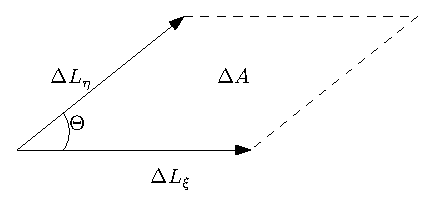
\includegraphics{fig/area.eps}
    \caption{Área}
    \label{fig:area}
\end{figure}

\begin{equation*}
    \Delta \vec{A} =
    \begin{vmatrix}
        \hat{i} & \hat{j} & \hat{k}\\
        x_\xi \Delta \xi & y_\xi \Delta \xi & 0\\
        x_\eta \Delta \eta & y_\eta \Delta -\eta & 0
    \end{vmatrix}
    = (x_\xi \Delta \xi y_\eta \Delta \eta - x_\eta \Delta \eta y_\xi \Delta \xi)\hat{k}
\end{equation*}

Assim:

\begin{equation*}
    \Delta A = x_\xi y_\eta \Delta \xi \Delta \eta - x_\eta y_\xi \Delta \xi \Delta \eta
\end{equation*}
\begin{equation*}
    \Delta A = (x_\xi y_\eta - x_\eta y_\xi)\Delta \xi \Delta \eta = J^{-1} \Delta \xi \Delta \eta\\
\end{equation*}    
\begin{equation}
    \label{eq:2.15}
    \Delta A = \frac{\Delta \xi \Delta \eta}{J}
\end{equation}

No caso tridimensional, pode-se provar que o volume físico $(\Delta v)$ é dado por:
\begin{equation}
    \label{eq:2.16}
    \Delta v = \frac{\Delta \xi \Delta \eta \Delta \gamma}{J}
\end{equation}

Sendo o jacobiano dado por:

\begin{equation}
    \label{eq:2.17}
    J = [x_\xi(y_\eta z_\gamma - y_\gamma z_\eta) - x_\eta(y_xi z_\gamma - y_\gamma z_\xi) + x_\gamma(y_\xi z_\eta - y_\eta z_\xi)]^{-1}
\end{equation}

\section{Tensor métrico 2D}

O Tensor métrico 2D é definido como:

\begin{equation}
    \label{eq:2.18}
    [g_{ij}] =
    \begin{vmatrix}
        g_{11} & g_{12}\\
        g_{21} & g_{22}
    \end{vmatrix}
    =
    \begin{vmatrix}
        \gamma & \beta\\
        \beta & \alpha
    \end{vmatrix}
\end{equation}

Em que:

\begin{equation}
    \label{eq:2.19}
    \beta = x_\xi x_\eta + y_\xi y_\eta
\end{equation}

Pode-se mostrar que o determinante do tensor métrico $g$ é dado por:

\begin{equation}
    \label{eq:2.20}
    g = \frac{1}{J^2}
\end{equation}

Das equações \ref{eq:2.20} e \ref{eq:2.18}, tem-se que:

\begin{equation*}
    \alpha \gamma - \beta^2 = \frac{1}{J^2}
\end{equation*}

E da equação \ref{eq:2.15}:

\begin{equation*}
    J=\frac{\Delta \xi \Delta \eta}{\Delta A}
\end{equation*}


Nesse caso,

\begin{equation*}
    \alpha \gamma - \beta^2 = \frac{\Delta A^2}{\Delta \xi^2 \Delta \eta^2}
\end{equation*}

Logo:

\begin{equation*}
    \Delta A^2 = (\alpha \gamma - \beta^2)\Delta \xi^2 \Delta \eta^2
\end{equation*}

Contudo,

\begin{equation*}
    \Delta A = \Delta L_\xi \Delta L_\eta \sin{\Theta} = \Delta \xi \sqrt{\gamma} \Delta \eta \sqrt{\alpha} \sin{\Theta}
\end{equation*}

Então:
\begin{equation*}
    \Delta A^2 = \Delta \xi^2 \gamma \Delta \eta^2 \alpha \sin{\Theta}^2
\end{equation*}

Igualando-se as expressões para $\Delta A^2$:
\begin{equation*}
    (\alpha \gamma - \beta^2)\Delta\xi^2 \Delta \eta^2 = \Delta \xi^2 \gamma \Delta \eta^2 \alpha \sin{\Theta}^2
\end{equation*}
\begin{equation*}
    \alpha \gamma - \beta^2 = \alpha \gamma \sin{\Theta}^2
\end{equation*}
\begin{equation*}
    \alpha \gamma(1-\sin{\Theta}^2) = \beta^2
\end{equation*}
\begin{equation*}
    \alpha \gamma \cos{\Theta}^2 = \beta^2
\end{equation*}

Ou seja:
\begin{equation}
    \label{eq:2.21}
    \beta = \sqrt{\alpha \gamma}\cos{\Theta}
\end{equation}

No caso de sistema ortogonais, $\Theta = \pi/2 = 90º$ e, portanto, $\beta = 0$. Deste modo, $\beta$ representa a não-ortogonalidade do sistema de coordenadas curvilíneas. O valor de $\Theta$ pode ser obtido para qualquer volume de controle ou malha, uma vez que ele é função de $\alpha, \beta$ e $\gamma$ que são funções das métricas.

\section{Vetores de base covariantes}
São os vetores tangentes às linhas de $\xi$ e $\eta$.

Conforme a figura \ref{fig:e_xi} tem-se que:

\begin{equation}
    \label{eq:2.22}
    \vec{r} = x \hat{i} + y \hat{j}
\end{equation}

\begin{figure}[h]
    \centering
    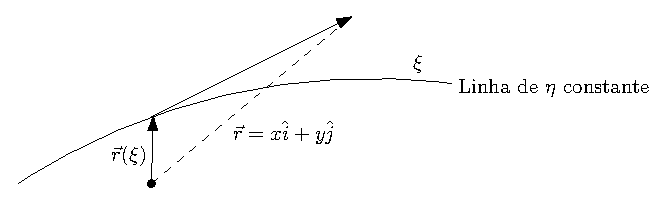
\includegraphics{fig/e_xi.eps}
    \caption{Definição de $e_\xi$}
    \label{fig:e_xi}
\end{figure}

\begin{equation}
    \label{eq:2.23}
    \vec{e_\xi} = \lim_{\Delta \xi \to 0} \frac{\vec{r}(\xi + \Delta \xi) - \vec{r}(\xi)}{\Delta \xi} = \frac{\partial \vec{r}}{\partial \xi}
\end{equation}

Portanto,

\begin{equation}
    \label{eq:2.24}
    \vec{e_\xi} = x_\xi \hat{i} + y_\xi \hat{j}
\end{equation}

que é tangente à linha de $\eta$ constante e analogamente:

\begin{equation}
    \label{eq:2.25}
    \vec{e_\eta} = x_\eta \hat{i} + y_\eta \hat{j}
\end{equation}

que é tangente à linha de $\xi$ constante.

Nota-se que, como $\hat{i}$ e $\hat{j}$ são unitários, $\vec{e_\xi}$ e $\vec{e_\eta}$ não o são.

\begin{equation}
    \label{eq:2.26}
    \vec{e_\xi} \cdot \vec{e_\xi} = x_\xi^2 + y_\xi^2 = \gamma
\end{equation}

\begin{equation}
    \label{eq:2.27}
    \vec{e_\eta} \cdot \vec{e_\eta} = x_\eta^2 + y_\eta^2 = \alpha
\end{equation}

\begin{equation}
    \label{eq:2.28}
    \vec{e_\xi} \cdot \vec{e_\eta} = x_\xi x_\eta + y_\xi y_\eta = \beta
\end{equation}

Como já mensionado, se $\beta = 0$, o sistema é ortogonal.